\section{Possible Performance Gains from Model Fragmentation}
\label{sec:gains}

In this section, we analyze the theoretically possible execution times of partially loading models with fragmentations of different granularity. This includes an assessments for performance gains from optimal fragmentation strategies compared to no or total fragmentation.

To keep this analysis simple, we have to make two assumptions that will probably seldom hold in reality, but still lead to analysis results that provide reasonable upper bounds for possible gains.
The first assumption: we are only consider fragmentations where all fragments have the same size $f$. 
This means a fragmentation for a model of size $m$ consist of $\lceil m/f \rceil$ fragments\footnote{$\lceil x\rceil$ denotes the ceiling of $x$}. 
The second assumption: all fragmentations are optimal regarding partial loads. This means to load a model part of size $l$, we only need to load $\lceil l/f\rceil$ fragments at most.

To determine the execution time for partial loading depending on the parameters model size $m$, fragment size $f$ and size of the model part $l$, we need two functions that determine the time it takes to read and parse a model and to access a value in a key value store. The read and parse function is linear depending on parsed model size $s$: $parse(s)=\mathcal{O}\left(s\right)$, the access function is logarithmic depending on the number of keys $k$: $access(k)=\mathcal{O}(log(k))$. Most key-value stores, including HBase (that we use for our implementations) provide $\mathcal{O}(log)$ accesses complexity (ref. also to Fig.~\ref{fig:hbaseAccessPerf}).

With the given assumptions, parameters, and functions the time to execute a partial load is:

$$t_{m,f}(l)=\overbrace{\left\lceil\frac{l}{f}\right\rceil}^{\mathclap{\text{number of fragments to load}}}\underbrace{\left(access(\left\lceil\frac{m}{f}\right\rceil) + parse(f)\right)}_{\mathclap{\text{time to load one fragment}}}$$

To actually use this cost function, we need concrete values for $parse$ and $access$. We measured the execution times for $parse$ with EMF's XMI parser for models of various sizes and fit a linear functions to the measured values (Fig.~\ref{fig:emfParsePerf}). For $access$ we measured the execution time for accessing keys in HBase for database tables with various numbers of keys $k$. For $k<10^6$ we use a linear function and for $k\ge 10^6$ a logarithmic function as a fit (Fig.~\ref{fig:hbaseAccessPerf}). 
%For details on the measuring environment refer to section~\ref{sec:evaluation}.

\begin{figure}[bt]
\begin{minipage}[b]{0.48\linewidth}
\centering
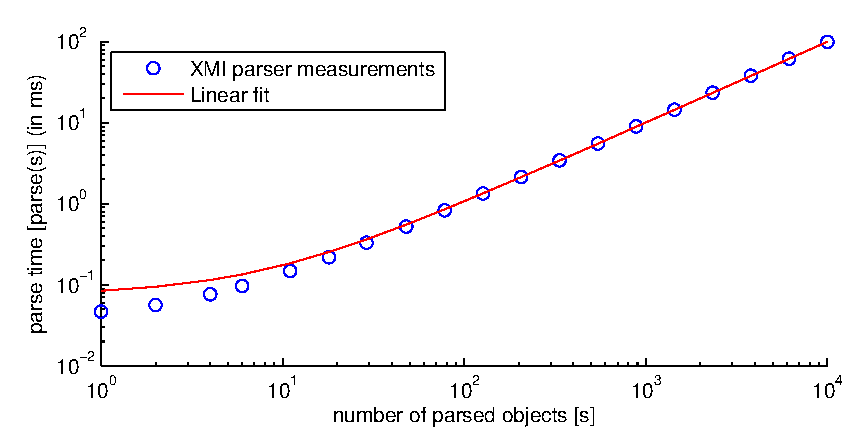
\includegraphics[width=\linewidth]{figures/emfParsePerf}
\caption{EMF's XMI parser performance.}
\label{fig:emfParsePerf}
\end{minipage}
\hspace{0.02\linewidth}
\begin{minipage}[b]{0.48\linewidth}
\centering
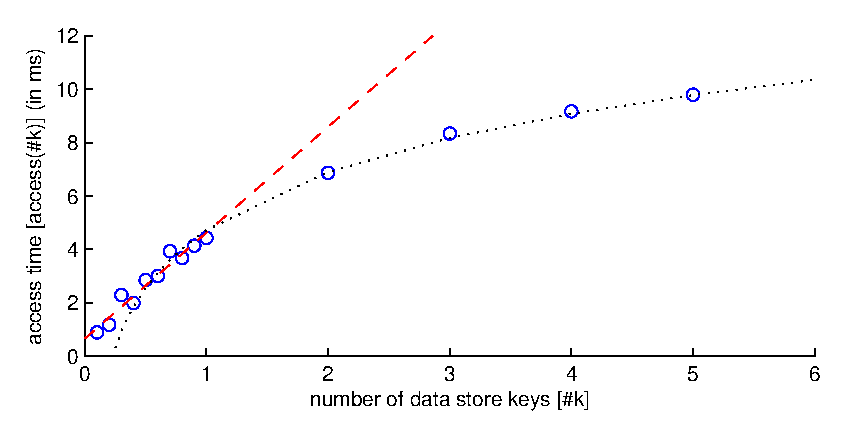
\includegraphics[width=\linewidth]{figures/hbaseAccessPerf}
\caption{HBase accesses performance.}
\label{fig:hbaseAccessPerf}
\end{minipage}
\end{figure}

 
Now, we can discuss the influence of fragment size $f$ on $t_{m,f}(l)$. First, we use a model of size $m=10^6$ and vary $f\in\{10^0,\dots,10^6\}$. Fig.~\ref{fig:theoryTimesSmall} shows the computed times $t$ over loaded model objects $l$ for the different fragment sizes $f$. We can observe four things. First, there is no optimal fragment size. Depending on the number of loaded objects, different fragment sizes are optimal. But intermediate fragment sizes provide good performance. With fragment size $f=10^2$ for example, all partial loads take three times the optimal time at most. Second, total fragmentation ($f=1$) requires roughly 100 times more time than optimal fragmentation, when larger numbers of objects $\ge 10^2$ are loaded. Thirdly, no fragmentation ($f=m$) is only a time efficient option, if we need to load almost all of the model. But in those cases no fragmentation is usually not practical for memory issues. Fourthly, for small partial models total fragmentation is far better than no fragmentation, for large partial models no fragmentation provides better performance.

\begin{figure}
\centering
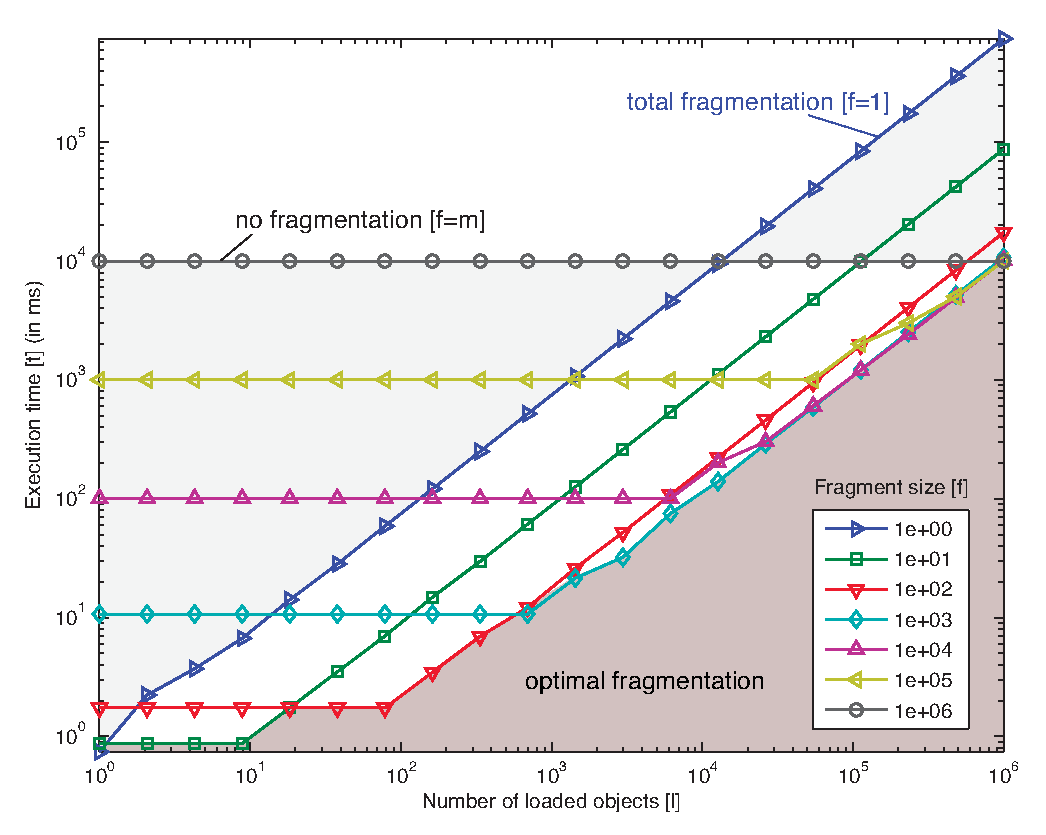
\includegraphics[width=0.65\linewidth]{figures/theoryTimesSmall}
\label{fig:theoryTimesSmall}
\caption{Computed execution times for partial loads from a model with $10^6$ objects and fragmentations of different granularity.}
\end{figure}

%Fig.~\ref{fig:theoryContour} shows the same data as contour plot. The largest partial models can be loading if the loaded parts have the same size as the fragments $l=f$. Fig.~\ref{fig:theoryTimesLarge} shows times for a larger model with $m=10^9$. Intermediate fragment sizes are still good fragment sizes. Such large models produce large number of database keys for total fragmentation, but the parsing overhead $parse(0)>0$ has obviously an larger influence than growing access times. Thus the plot for total fragmentation is still a line, and for large number of loaded objects, the plot for all fragment sizes are parallel.

%\begin{figure}[b]
%\begin{minipage}[b]{0.48\linewidth}
%\centering
%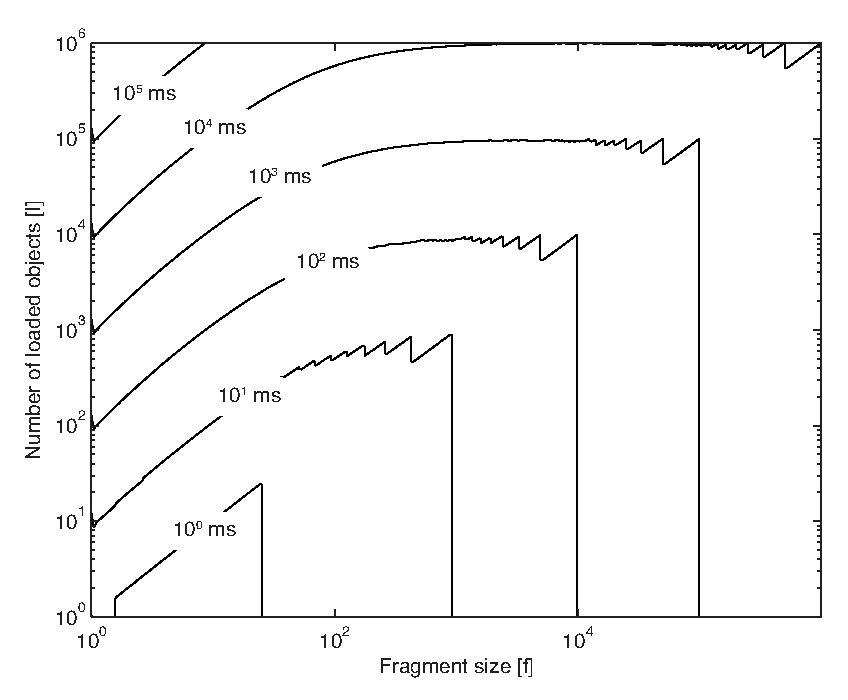
\includegraphics[width=\linewidth]{figures/theoryContour}
%\caption{Contour plot. Shows which $(f,l)$ have the same costs $t$.}
%\label{fig:theoryContour}
%\end{minipage}
%\hspace{0.02\linewidth}
%\begin{minipage}[b]{0.48\linewidth}
%\centering
%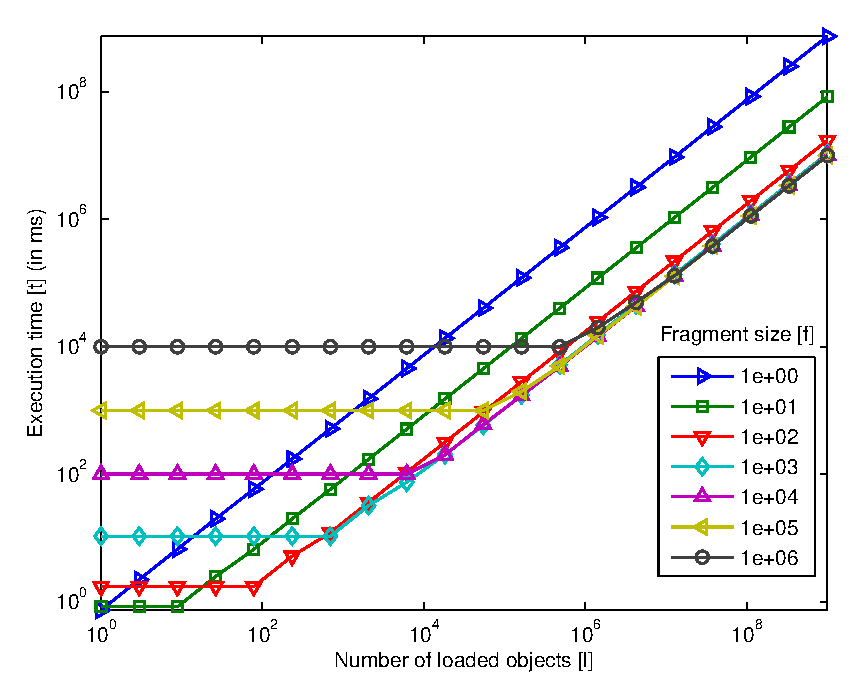
\includegraphics[width=\linewidth]{figures/theoryTimesLarge}
%\caption{Computed partial load times for a model of size $10^9$.}
%\label{fig:theoryTimesLarge}
%\end{minipage}
%\end{figure}